\documentclass[border=12pt]{standalone}
\usepackage{tikz}
\usetikzlibrary{shapes.geometric, arrows.meta, positioning, calc, fit, backgrounds}
\usepackage{fontspec}
\usepackage{amsmath,amssymb}
\setmainfont{DejaVu Sans}

\begin{document}
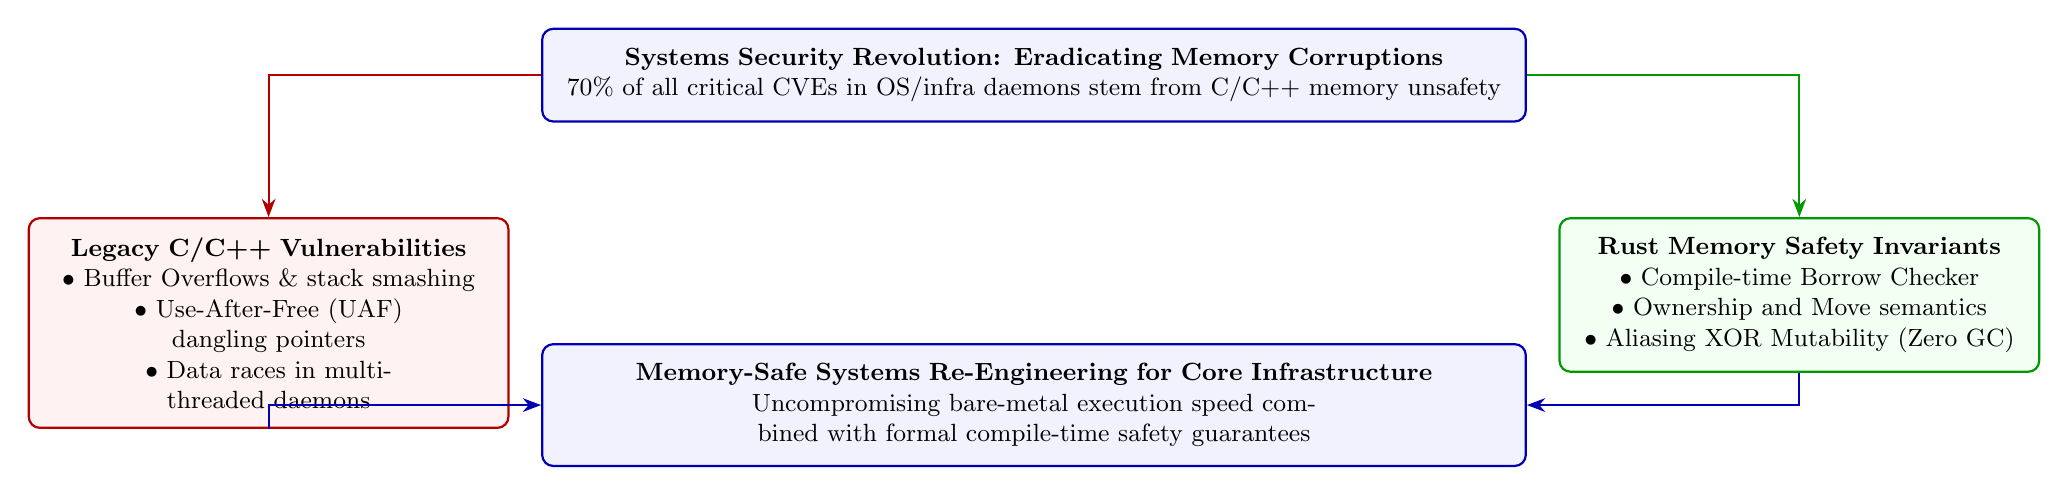
\begin{tikzpicture}[
    font=\small,
    >=Stealth,
    node distance=1.2cm,
    block/.style={rectangle, draw=blue!70!black, fill=blue!5, rounded corners=4pt, thick, align=center, inner sep=7pt},
    alertblock/.style={rectangle, draw=red!70!black, fill=red!5, rounded corners=4pt, thick, align=center, inner sep=7pt},
    greenblock/.style={rectangle, draw=green!60!black, fill=green!5, rounded corners=4pt, thick, align=center, inner sep=7pt},
    amberblock/.style={rectangle, draw=orange!80!black, fill=orange!5, rounded corners=4pt, thick, align=center, inner sep=7pt}
]

\node[block, text width=12cm] (top) {\textbf{Systems Security Revolution: Eradicating Memory Corruptions}\\70\% of all critical CVEs in OS/infra daemons stem from C/C++ memory unsafety};

\node[alertblock, below left=1.2cm and 0.4cm of top, text width=5.6cm] (c_bugs) {\textbf{Legacy C/C++ Vulnerabilities}\\$\bullet$ Buffer Overflows \& stack smashing\\$\bullet$ Use-After-Free (UAF) dangling pointers\\$\bullet$ Data races in multi-threaded daemons};

\node[greenblock, below right=1.2cm and 0.4cm of top, text width=5.6cm] (rust) {\textbf{Rust Memory Safety Invariants}\\$\bullet$ Compile-time Borrow Checker\\$\bullet$ Ownership and Move semantics\\$\bullet$ Aliasing XOR Mutability (Zero GC)};

\node[block, below=2.8cm of top, text width=12cm] (bottom) {\textbf{Memory-Safe Systems Re-Engineering for Core Infrastructure}\\Uncompromising bare-metal execution speed combined with formal compile-time safety guarantees};

\draw[->, thick, red!70!black] (top) -| (c_bugs);
\draw[->, thick, green!60!black] (top) -| (rust);
\draw[->, thick, blue!70!black] (c_bugs) |- (bottom);
\draw[->, thick, blue!70!black] (rust) |- (bottom);

\end{tikzpicture}
\end{document}
